\documentclass[a4paper,UTF8]{article}

\usepackage[margin=1.25in]{geometry}
\usepackage{color}
\usepackage{graphicx}
\usepackage{amssymb}
\usepackage{amsmath}
\usepackage{amsthm}
\usepackage{enumerate}
\usepackage{bm}
\usepackage{hyperref}
\usepackage{epsfig}
\usepackage{color}
\usepackage{mdframed}
\usepackage{lipsum}
\usepackage{mathtools}
\usepackage{algorithm}
\usepackage{algorithmic}
\usepackage{listings}
\usepackage{xcolor}
\usepackage{float}
\usepackage{caption}

\usepackage[utf8]{inputenc}
\usepackage[UTF8]{ctex}

\newmdtheoremenv{thm-box}{myThm}
\newmdtheoremenv{prop-box}{Proposition}
\newmdtheoremenv{def-box}{define}

\setlength{\evensidemargin}{.25in}
\setlength{\textwidth}{6in}
\setlength{\topmargin}{-0.5in}
\setlength{\topmargin}{-0.5in}

\usepackage{indentfirst}
\setlength{\parindent}{2em}

\usepackage{subfigure}
% \setlength{\textheight}{9.5in}
%%%%%%%%%%%%%%%%%%set header and footer here%%%%%%%%%%%%%%%%%%
\usepackage{fancyhdr}
\usepackage{lastpage}
\usepackage{layout}
\footskip = 10pt
\pagestyle{fancy}
\lhead{2020, Spring}
\chead{大数据综合处理实验}
\rhead{实验三}
\cfoot{\thepage}
\renewcommand{\headrulewidth}{1pt}  			%header
\setlength{\skip\footins}{0.5cm}    			
\renewcommand{\footrulewidth}{0pt}  		

\makeatletter 							
\def\headrule{{\if@fancyplain\let\headrulewidth\plainheadrulewidth\fi%
\hrule\@height 1.0pt \@width\headwidth\vskip1pt	
\hrule\@height 0.5pt\@width\headwidth  			
\vskip-2\headrulewidth\vskip-1pt}      			
 \vspace{6mm}}     						
\makeatother

\graphicspath{{img/}}

\lstset{
 columns=fixed,
 basicstyle = \footnotesize,
 breakatwhitespace=false,         % 设置是否当且仅当在空白处自动中断.
 breaklines=true,
 numbers=left,                                        % 在左侧显示行号
 numberstyle=\tiny\color{gray},                       % 设定行号格式
 frame=none,                                          % 不显示背景边框
 backgroundcolor=\color[RGB]{245,245,244},            % 设定背景颜色
 keywordstyle=\color[RGB]{40,40,255},                 % 设定关键字颜色
 numberstyle=\footnotesize\color[RGB]{96,96,96},
 commentstyle=\color[RGB]{0,128,0},                % 设置代码注释的格式
 stringstyle=\rmfamily\slshape\color[RGB]{128,0,0},   % 设置字符串格式
 showstringspaces=false,                              % 不显示字符串中的空格
 language=JAVA,
 extendedchars=true,
 escapeinside=''                                       % 设置语言
}

%%%%%%%%%%%%%%%%%%%%%%%%%%%%%%%%%%%%%%%%%%%%%%
\numberwithin{equation}{section}
\newtheorem{myThm}{myThm}
\newtheorem*{myDef}{Definition}
\newtheorem*{mySol}{Solution}
\newtheorem*{myProof}{Proof}
\newcommand{\indep}{\rotatebox[origin=c]{90}{$\models$}}
\newcommand*\diff{\mathop{}\!\mathrm{d}}

\usepackage{multirow}
\renewcommand\refname{reference}
\author{组长:韩畅,组员:李展烁、王一之、闫旭芃}
\begin{document}
%hello world
%\listoffigures
\captionsetup[figure]{labelfont={bf},labelformat={default},labelsep=period,name={图}}
\title{大数据综合处理实验\\
实验三}
\maketitle

\section{实验规划与设计}
\subsection{任务分配}
{171860551, \text{韩畅:组长,项目规划,算法设计,程序框架及大部分功能,程序初步运行、优化}}\\ \indent
{171860550, \text{王一之:算法设计,代码管理,报告撰写,代码注释添加、整理}}\\ \indent
{171860549, \text{闫旭芃:算法设计,完善代码功能,添加代码注释,报告主体撰写}}\\ \indent
{171840565, \text{李展烁:算法设计,程序集群运行、调试、优化}}
\subsection{任务要求}
使用 MapReduce 完成两张表的 join 操作,存入到 Hive 中。
\subsection{设计思路}
实现两张表的join操作,可以利用mapreduce的特性,读入order和product将两张表到map中,
将key打包成自定义的数据类型输出,并且按照两表中关联的条件排序依据,
将两表满足join条件的数据并携带数据所来源的文件信息,发往同一个reduce task,在reduce中进行数据的串联
\begin{figure}[H]
    \centering

    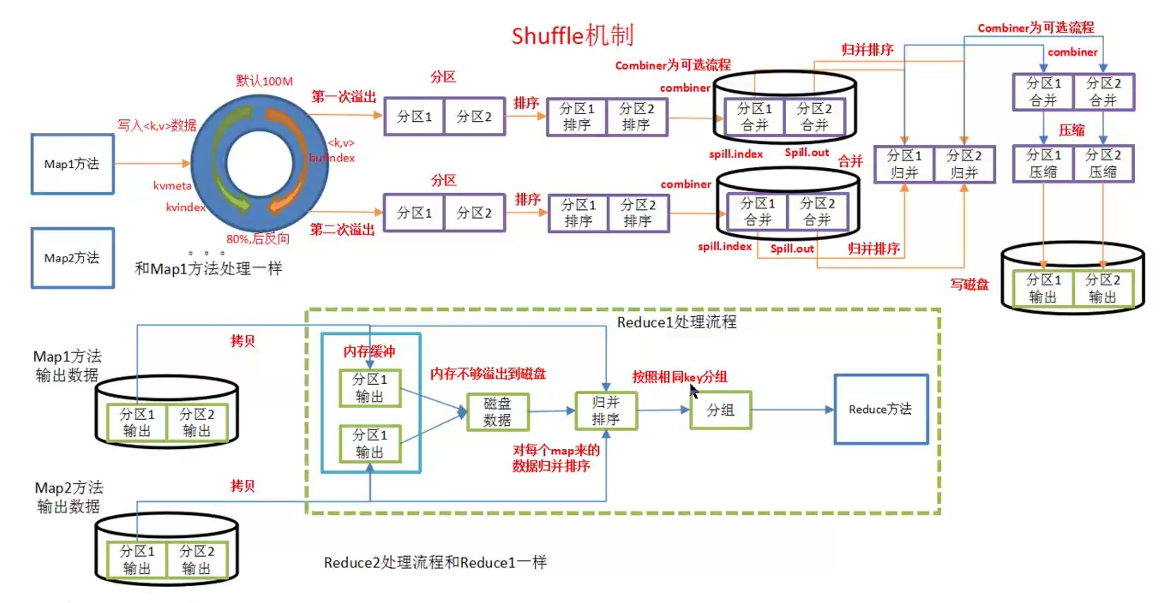
\includegraphics[width = 15cm]{shuffle.png}

    \caption{mapreduce shuffle工作流程图}
\end{figure}
\subsubsection{自定义数据类型}
自定义一个bean存储表中每一种数据:oid,odata,oamount,pid,pname,price
\begin{figure}[H]
    \centering

    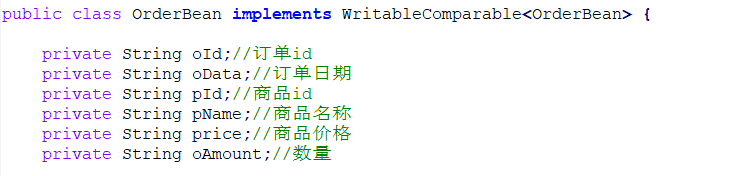
\includegraphics[width = 15cm]{bean1.png}

    \caption{自定义bean}
\end{figure}
实现一些必要的函数,并且实现compareTo(),目的是为了按照pid进行排序分组,每一组然后按照pname排序,因为o表中不存在pname所以,p表中的内容就会被排在o表内容的前面
\begin{figure}[H]
    \centering
    \subfigure[实现compareTo]
    {
        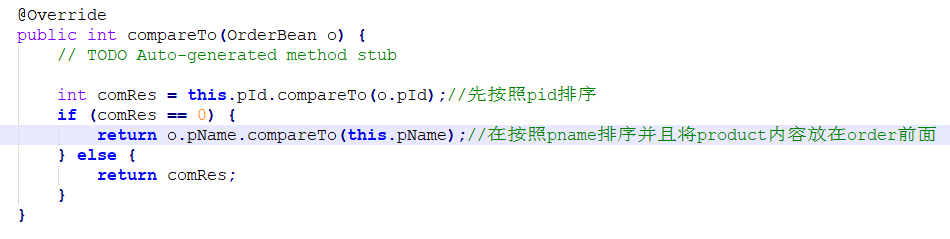
\includegraphics[width = 15cm]{bean2.png}
    }
    \vfill
    \subfigure[部分其他函数(1)]
    {
        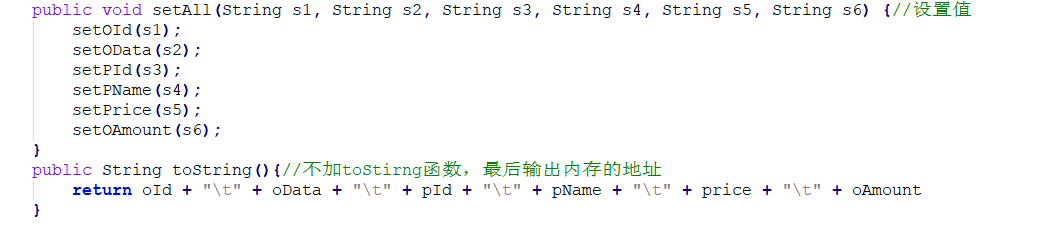
\includegraphics[width = 15cm]{bean3.png}
    }
    \vfill
    \subfigure[部分其他函数(2)]
    {
        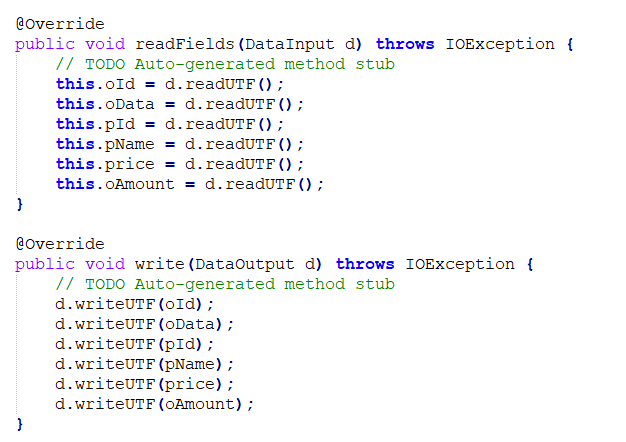
\includegraphics[width = 15cm]{bean4.png}
    }

    \caption{orderbean部分代码实现}
\end{figure}
\subsubsection{主功能Map设计思路}
分辨读入的数据来源于哪个文件,分别给相应的值赋值,不存在的值则赋值为空。输出的key打包成之前自定义的ordebean类型
\begin{figure}[H]
    \centering

    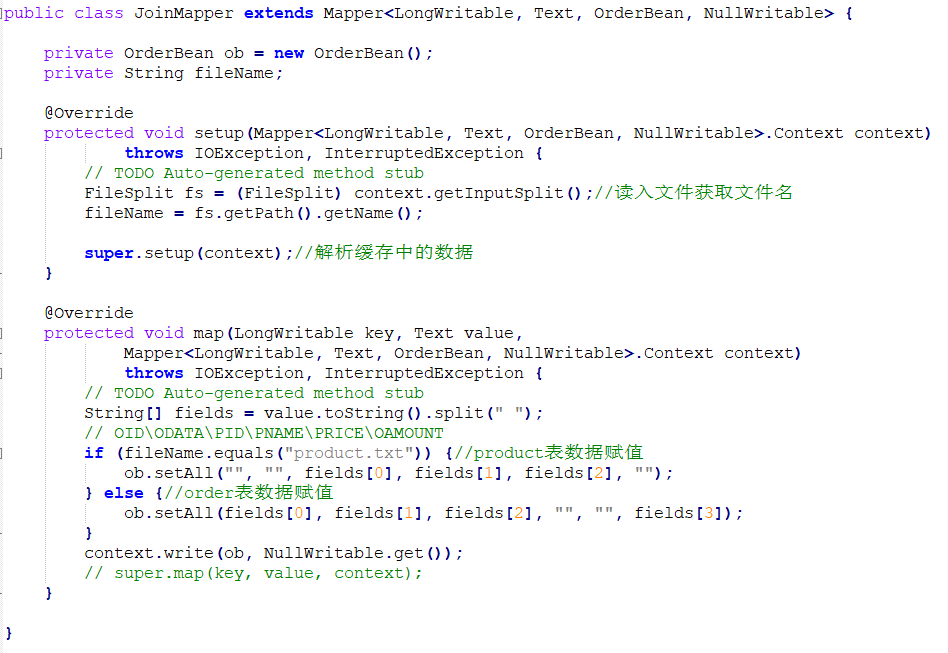
\includegraphics[width = 15cm]{map1.png}

    \caption{Mapper部分实现}
    \label{mapper}
\end{figure}
\subsubsection{重写Partitioner}
对map发出的数据进行分区,根据pid进行分区
\begin{figure}[H]
    \centering

    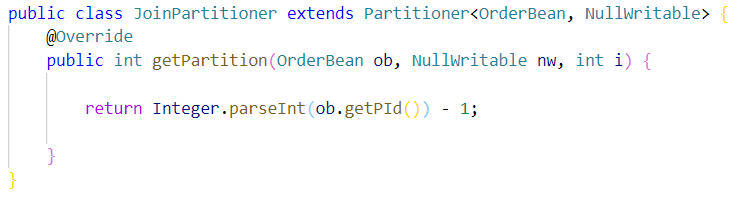
\includegraphics[width = 15cm]{part1.png}

    \caption{Partitioner部分实现}
\end{figure}
\subsubsection{排序}
排序会根据key排序,由于key是自定义数据类型orderbean,所以在orderbean中需要自定义排序方法(见上)\\
compareTo函数首先按照pid排序,然后按照pname排序。由于product中pid 是唯一的,所以相同的pid中只会有一个pname,并且会被排序到最前面,形成特定的结构
\begin{figure}[H]
    \centering
    \subfigure[按照pid进行排序]
    {
        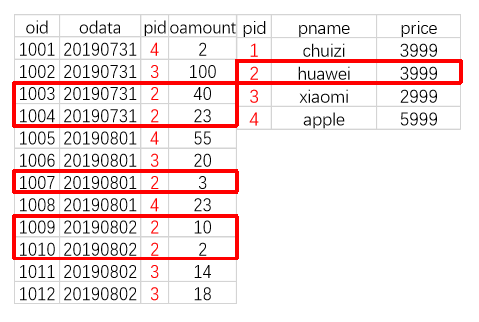
\includegraphics[width = 14cm]{ord1.png}
    }
    \vfill
    \subfigure[排序结果示例]
    {
        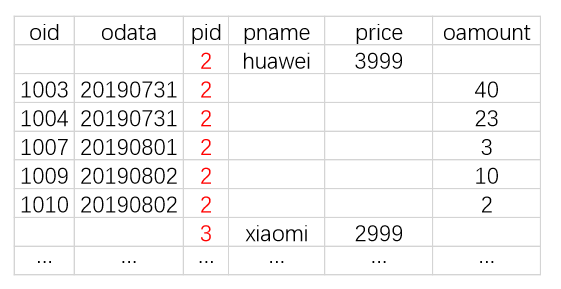
\includegraphics[width = 14cm]{ord2.png}
    }
    \caption{排序示例}
\end{figure}
\subsubsection{自定义分组}
一个reduce任务,默认只会接收到一个key的数据,所以我们要把相同pid的数据分到一个组里面处理
\begin{figure}[H]
    \centering

    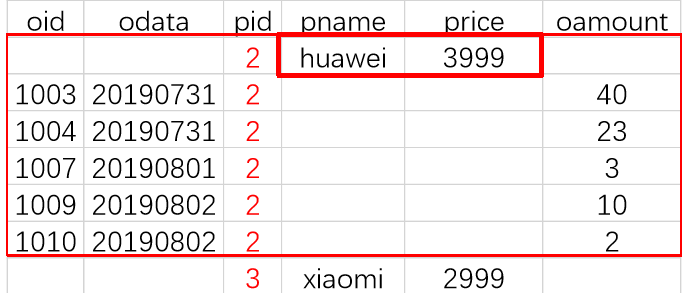
\includegraphics[width = 15cm]{comp1.png}

    \caption{自定义分组示例}
\end{figure}
\begin{figure}[H]
    \centering

    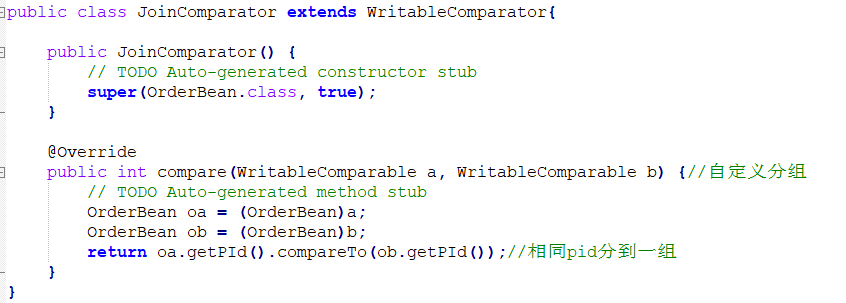
\includegraphics[width = 15cm]{comp2.png}

    \caption{重写Comparator}
\end{figure}
\subsubsection{主功能Reduce设计思路}
输入的第一对中的key为要join的对应的Pname及Price,将此值分别赋给之后的所有键值对中的key,并写入结果。
\begin{figure}[H]
    \centering

    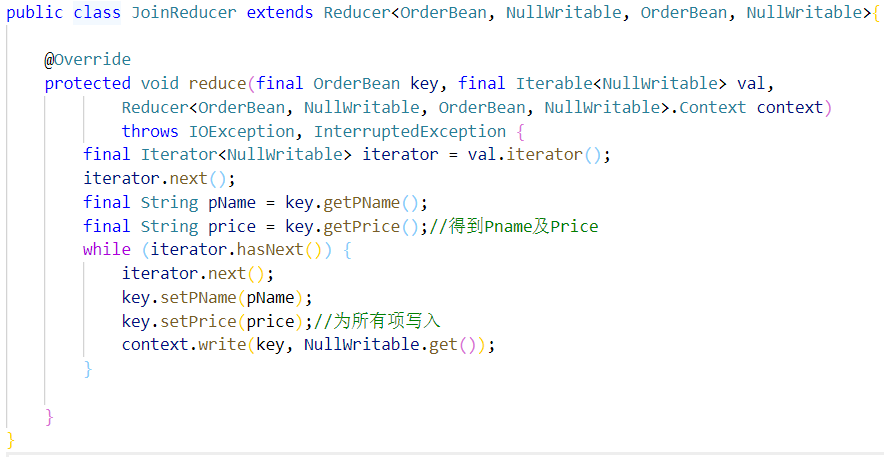
\includegraphics[width = 15cm]{reducer.png}

    \caption{重写Reducer}
    \label{reducer}
\end{figure}

\subsubsection{Key-Value类型协调}
value设为空NullWritable,自定义key数据类型OrderBean,将数据全部封装到这里面,方便后续排序,分区,分组
\subsection{代码演示}
\subsubsection{Map阶段代码演示}
已经包含在设计思路图片中,见图\ref{mapper}

\subsubsection{Reduce阶段代码演示}
同上,见图\ref{reducer}
\section{实验结果展示}

\subsection{结果文件在HDFS上的路径}
/user/2020st18/output2/
\subsection{所有命令}
jar包执行命令:hadoop jar /home/2020st18/HiveMyJoin.jar MyJoin.JoinDriver /data/exercise\_3 output2 

hive建表命令:create table orders(id int,order\_date string,pid string,name string,price int,num int) row format delimited fields terminated by '\t' location '/user/2020st18/output2/';
\subsection{hive 输出结果文件的部分截图}
\begin{figure}[H]
	\centering
	\subfigure[orders表开头]
	{
		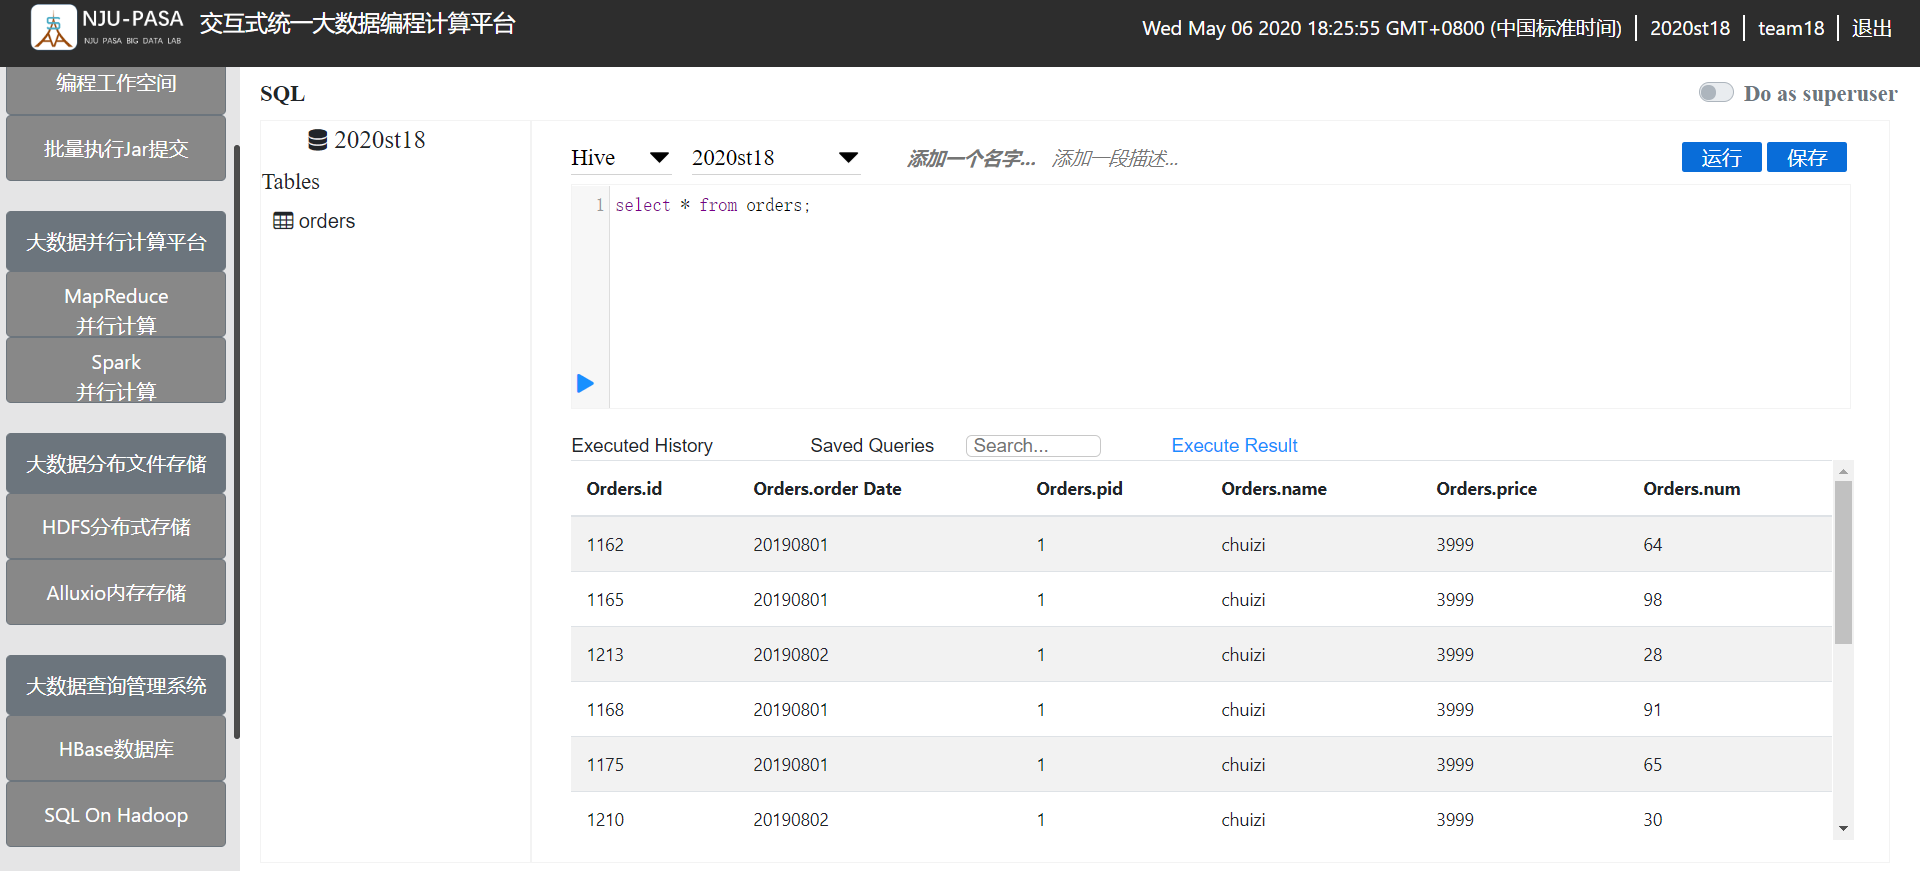
\includegraphics[width = 15cm]{hive1.PNG}
	}
	\vfill
	\subfigure[orders表结尾]
	{
		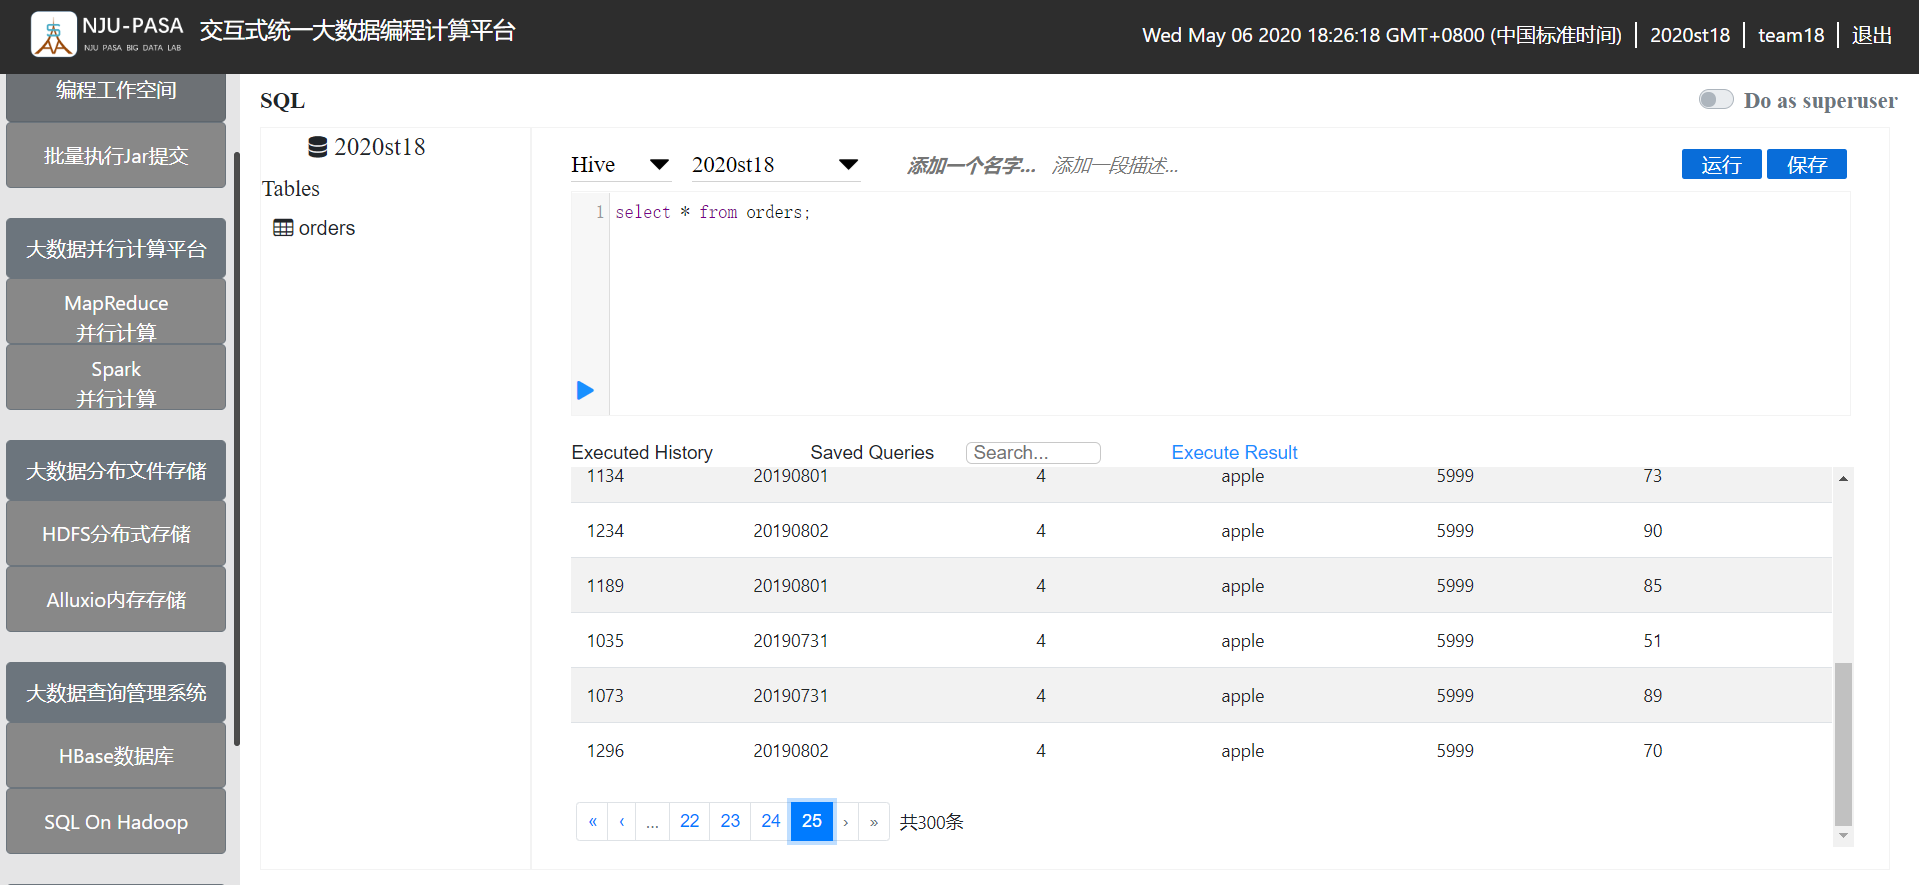
\includegraphics[width = 15cm]{hive2.PNG}
	}
	
	\caption{Hive执行结果}
\end{figure}

\subsection{Web UI 报告内容展示}
\begin{figure}[H]
	\centering
	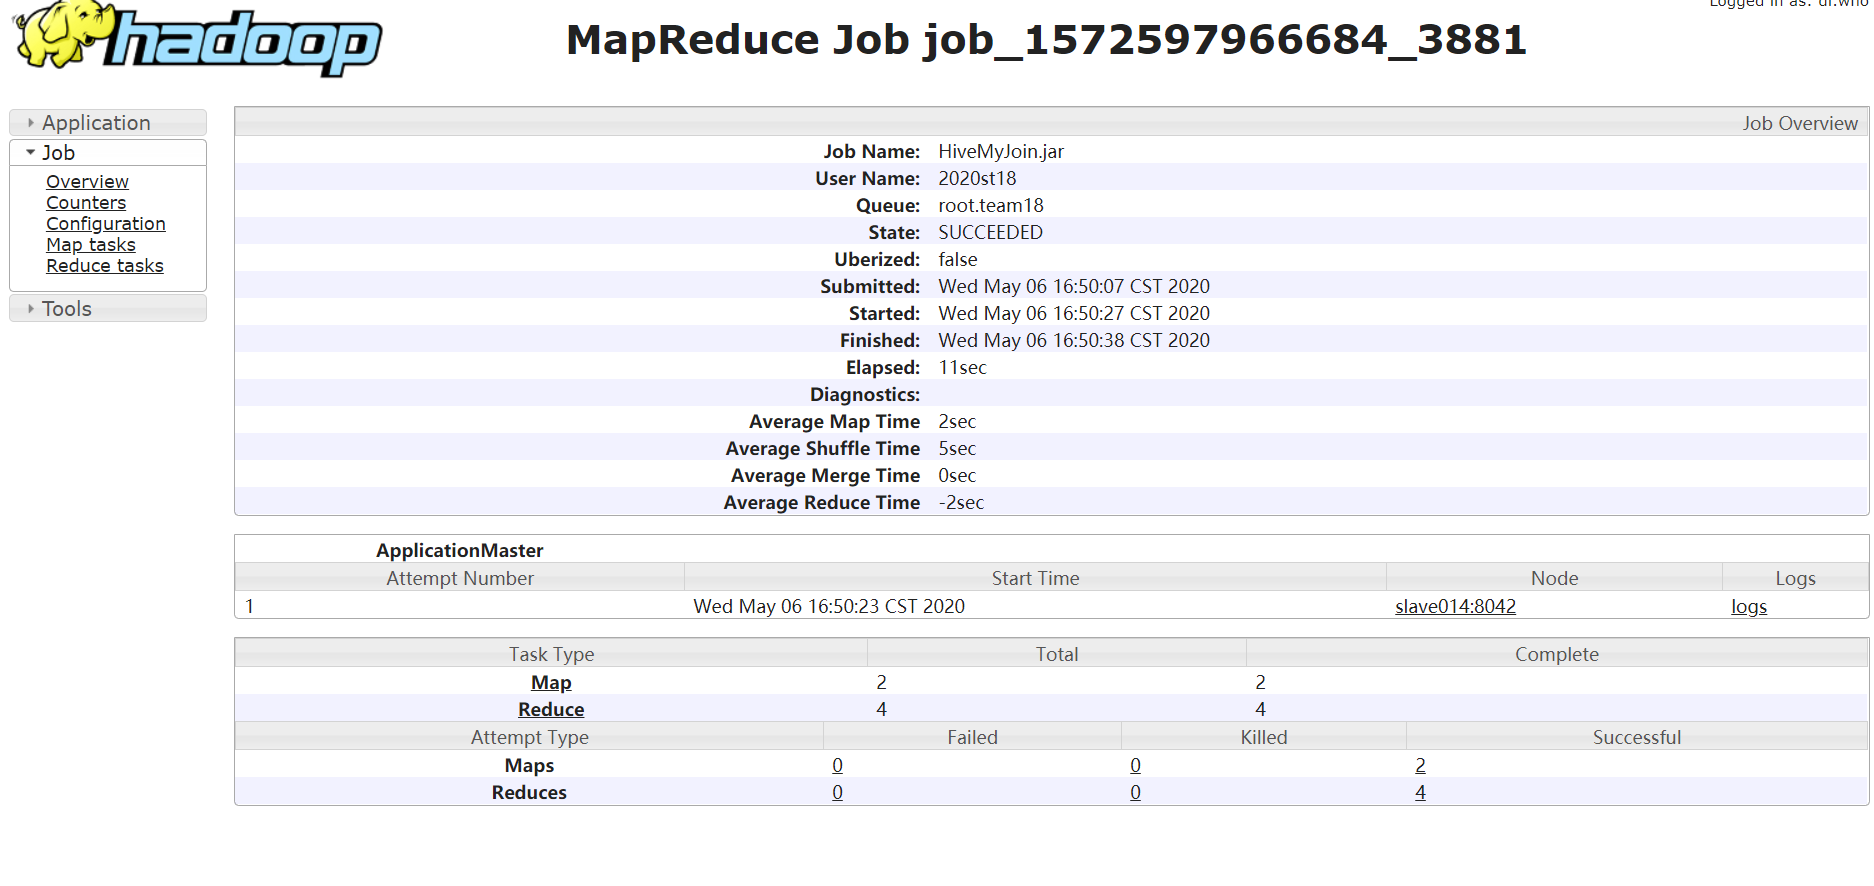
\includegraphics[width = 15cm]{job.PNG}
	\caption{WebUI执行报告}
\end{figure}
\section{实验经验总结与改进方向}
\begin{itemize}
	\item 同上次实验相比,使用github进行版本管理与协作,提高了效率
	\item 利用了reducer中values调用next()时key也同步更新的特性,进行reducer设计
\end{itemize}

\bibliographystyle{plain}
\bibliography{ref}

\end{document}
